% Provenance (never printed): see sources/outline_sources.md (Year 3:
% geophysical fluid dynamics: rotating-frame equations, Rossby number,
% hydrostatic and geostrophic balance, thermal wind, buoyancy frequency).
% Brief: sources/book5/BRIEFS.md, ch. 19. Curves from
% figdata/bachelor-3/inertial_oscillation.py, thermal_wind.py and
% buoyancy_frequency.py. Exercise and problem values in the Book 5 scratch
% calculator calc/ch19.py. The Steppe of Orrin, its lake, its stations and
% its winds are invented.
\chapter{भू-भौतिकीय द्रव गतिकी}\label{ch:b3:gfd-foundations}

चाय का एक प्याला हिलाइए तो घुमाव एक मिनट में शांत हो जाता है; पत्तियाँ
प्याले के तल के बीच में इकट्ठी हो जाती हैं, और उसके अलावा कुछ नहीं होता।
महासागर और वायुमंडल को भी सूर्य और पवन हिलाते हैं, परंतु वे घूर्णन करते ग्रह पर
और विभिन्न घनत्व की परतों में होते हैं। घूर्णन और स्तरीकरण उन्हें ऐसे नियमों का पालन कराते हैं
जो चाय के प्याले में कभी नहीं दिखते: पवनें समदाब रेखाओं के पार नहीं, बल्कि उनके साथ-साथ बहती हैं,
द्रव के स्तंभ झुकने से इनकार करते हैं, और ऊपरी क्षोभमंडल की पवन
उसके नीचे के तापमानों में लिखी होती है। इस अध्याय में इन बड़े, धीमे और पतले प्रवाहों के समीकरण स्थापित किए जाते हैं
और वे कुछ संख्याएँ, जो तय करती हैं
कि कौन-से पद महत्त्वपूर्ण हैं।

\begin{recall}
घूर्णनशील तंत्र में कोरिऑलिस और अपकेंद्री बल, नेवियर–स्टोक्स और सांतत्य समीकरण,
श्यानता, रेनॉल्ड्स संख्या और द्रवस्थैतिक संबंध भौतिकी की पुस्तकों में हैं।
कोरिऑलिस प्राचल $f = 2\Omega
\sin\varphi$, दाब-प्रवणता बल, भू-विक्षेपी संतुलन, भू-विक्षेपी और प्रवणता पवनें
तथा जेट धाराएँ पुस्तक 3 (स्नातक वर्ष 1) में हैं,
उसके उस अध्याय में जो वायुमंडल के सामान्य परिसंचरण पर है;
एकमन परत उसके उस अध्याय में जो महासागर के परिसंचरण पर है;
विभव तापमान, स्थैतिक स्थिरता और उठाए गए वायु-पिंड का दोलन उसके उस अध्याय में है
जो वायुमंडल और महासागर की संरचना पर है।
\end{recall}

\section{घूर्णनशील तंत्र में समीकरण}\label{sec:b3:gfd-foundations:equations}

पृथ्वी के साथ घूमने वाले तंत्र में, कोणीय वेग
$\vec\Omega$ पर, वेग $\vec u$ वाला द्रव-पिंड इस समीकरण का पालन करता है
\[
\frac{\mathrm D\vec u}{\mathrm Dt} + 2\vec\Omega\times\vec u =
-\frac{1}{\rho}\nabla p + \vec g + \nu\nabla^2\vec u ,
\qquad
\frac{\partial\rho}{\partial t} + \nabla\cdot(\rho\vec u) = 0 ,
\]
जहाँ $\mathrm D/\mathrm Dt = \partial/\partial t + \vec u\cdot\nabla$
पिंड के साथ चलने वाला अवकलज है और $\nu$ गतिक श्यानता है। अपकेंद्री
बल गुरुत्वाकर्षण में जोड़ा गया है: इनका योग $\vec g$ प्रभावी गुरुत्व है,
जो \omterm{def:b3:gravity-geodesy:geopotential}{भू-विभव} के तल-पृष्ठों के लंबवत होता है, और ऊर्ध्वाधर दिशा इसी से परिभाषित होती है।
घूर्णन से केवल कोरिऑलिस पद, $-2\vec\Omega\times
\vec u$, शेष रहता है, और यह कोई कार्य नहीं करता: यह पिंड की चाल बदले बिना उसकी दिशा मोड़ता है।
पृथ्वी $\Omega =
\qty{7.292115e-5}{rad/s}$ से घूमती है, और एक नाक्षत्र दिवस \qty{23.9345}{h} का होता है।
% ledger: geod5:grs80-defining, earth:Trot

पृथ्वी की त्रिज्या $a$ से बहुत छोटी दूरियों पर होने वाली गति के लिए
स्थानीय कार्तीय तंत्र पर्याप्त है: $x$ पूर्व की ओर, $y$ उत्तर की ओर, $z$ ऊपर की ओर,
अक्षांश $\varphi$ पर, नीचे के चित्र का स्पर्श-समतल। वहाँ
$\vec\Omega = \Omega\,(0, \cos\varphi, \sin\varphi)$ है, और संवेग समीकरण के तीनों
घटक इस प्रकार हैं
\[
\begin{aligned}
\frac{\mathrm Du}{\mathrm Dt} - f v + \tilde f w &= -\frac{1}{\rho}\frac{\partial p}{\partial x} + F_x ,\\
\frac{\mathrm Dv}{\mathrm Dt} + f u &= -\frac{1}{\rho}\frac{\partial p}{\partial y} + F_y ,\\
\frac{\mathrm Dw}{\mathrm Dt} - \tilde f u &= -\frac{1}{\rho}\frac{\partial p}{\partial z} - g + F_z ,
\end{aligned}
\qquad f = 2\Omega\sin\varphi,\quad \tilde f = 2\Omega\cos\varphi ,
\]
जहाँ $\vec F$ घर्षण है। पतले, लगभग क्षैतिज प्रवाहों के लिए, जैसे
महासागर और वायुमंडल के, $\tilde f$ वाले पद छोड़ दिए जाते हैं: $\tilde f w$
$fv$ की तुलना में छोटा है, क्योंकि $w \ll v$ है, और $\tilde f u$ का मान
$g$ का दस-हज़ारवाँ भाग है (\cref{exo:b3:gfd-foundations:5} देखिए)। तब कोरिऑलिस बल केवल
क्षैतिज में कार्य करता है, घूर्णन के स्थानीय ऊर्ध्वाधर घटक
$\Omega\sin\varphi$ के माध्यम से।

\begin{definition}[$f$-समतल और $\beta$-समतल]\label{def:b3:gfd-foundations:planes}
संदर्भ अक्षांश $\varphi_0$ के निकट, \emph{$f$-समतल}\index{$f$-समतल}
सन्निकटन कोरिऑलिस प्राचल को स्थिर मानता है, $f = f_0 =
2\Omega\sin\varphi_0$। \emph{$\beta$-समतल}\index{$\beta$-समतल}
सन्निकटन उत्तर की ओर की दूरी $y$ के साथ इसका प्रथम-कोटि परिवर्तन रखता है:
$f = f_0 + \beta y$, जहाँ $\beta = \mathrm df/\mathrm dy = 2\Omega
\cos\varphi_0/a$ है।
\end{definition}

\ang{45} पर, माध्य त्रिज्या $a = \qty{6371}{km}$ के साथ, $f_0 =
\qty{1.031e-4}{s^{-1}}$ और $\beta = \qty{1.62e-11}{m^{-1}.s^{-1}}$ है:
\qty{1000}{km} के अक्षांश-विस्तार में $f$ में \qty{16}{\percent} परिवर्तन होता है।
$f$-समतल उससे बहुत छोटी गतियों के लिए उपयुक्त है; $\beta$-समतल
बेसिन-व्यापी धाराओं और ग्रहीय तरंगों के लिए आवश्यक होता है।
% ledger: earth:Rmean, geod5:grs80-defining (values in figdata/bachelor-3/inertial_oscillation.py)

\begin{omfigure}
\begin{minipage}[c]{0.42\linewidth}\centering
\begin{tikzpicture}[>=stealth, font=\small]
\draw[thick] (0,0) circle (2);
\draw[black!40, dashed] (-2,0) -- (2,0);
\draw[->, thick] (0,-2.4) -- (0,2.75) node[above] {$\vec\Omega$};
\draw (0,0) -- (30:2) coordinate (P);
\draw (0.6,0) arc (0:30:0.6);
\node at (15:0.9) {$\varphi$};
\draw[black!60] ($(P)+(120:-1.1)$) -- ($(P)+(120:1.3)$);
\draw[->, omThm, thick] (P) -- ++(0,1.6) node[right] {$\vec\Omega$};
\draw[->, omDef, thick] (P) -- ++(30:0.8) node[anchor=south west, align=left, inner sep=1pt] {$\Omega\sin\varphi$,\\ ऊपर};
\draw[->, omMeth, thick] (P) -- ++(120:1.386) node[anchor=south, align=center, inner sep=1pt] {$\Omega\cos\varphi$,\\ उत्तर};
\draw[black!50, densely dotted] ($(P)+(30:0.8)$) -- ($(P)+(0,1.6)$) -- ($(P)+(120:1.386)$);
\draw (P) circle (0.09); \draw ($(P)+(-0.064,-0.064)$) -- ($(P)+(0.064,0.064)$);
\draw ($(P)+(-0.064,0.064)$) -- ($(P)+(0.064,-0.064)$);
\node[font=\scriptsize, anchor=west] at ($(P)+(0.14,-0.03)$) {$x$, पूर्व};
\node[font=\scriptsize, black!60] at (-1.15,-0.25) {भूमध्य रेखा};
\end{tikzpicture}
\end{minipage}\hfill
\begin{minipage}[c]{0.55\linewidth}\centering
\begin{tikzpicture}
\begin{axis}[width=\linewidth, height=0.72\linewidth, xmin=0, xmax=90, ymin=0, ymax=1.8,
  xlabel={अक्षांश (\unit{\degree})}, ylabel={$f$ ($10^{-4}$\,\unit{s^{-1}})},
  xtick={0,15,30,45,60,75,90}, tick label style={font=\scriptsize}, label style={font=\small},
  legend style={font=\scriptsize, draw=none, fill=none}, legend pos=north west]
% computed in figdata/bachelor-3/inertial_oscillation.py
\addplot[omDef, thick] table[x=lat, y=f] {figdata/out/bachelor-3-inertial_oscillation-fbeta.dat};
\addplot[omThm, densely dashed] table[x=lat, y=fb] {figdata/out/bachelor-3-inertial_oscillation-fbeta.dat};
\addplot[only marks, mark=*, mark size=1.6pt] coordinates {(45,1.03126)};
\legend{$2\Omega\sin\varphi$, \ang{45} पर $\beta$-समतल}
\end{axis}
\end{tikzpicture}
\end{minipage}

\par\smallskip{\small बाईं ओर, अक्षांश $\varphi$ पर स्थानीय फ़्रेम: $z$
स्थानीय ऊर्ध्वाधर के अनुदिश, स्पर्शी समतल में $y$ उत्तर की ओर, $x$ पूर्व की ओर
पृष्ठ के भीतर की ओर। घूर्णन सदिश दो भागों में विभक्त होता है: $\Omega\sin\varphi$
ऊर्ध्वाधर के परितः, जो क्षैतिज गति को मोड़ता है, और
उत्तर की ओर की अक्ष के परितः $\Omega\cos\varphi$, जिसे पतले प्रवाहों के लिए छोड़ दिया जाता है। दाईं ओर कोरिऑलिस प्राचल और
\ang{45} पर इसकी $\beta$-समतल स्पर्शरेखा: अक्षांश की एक पट्टी पर यह निकट रहती है, और
भूमध्य रेखा तथा ध्रुव के निकट इससे दूर रहती है।}\label{fig:b3:gfd-foundations:frame}
\end{omfigure}
% ledger: geod5:grs80-defining, earth:Rmean

दो और सन्निकटन समीकरणों को सरल बनाते हैं, बिना उन बातों को खोए
जो मायने रखती हैं। पहला घनत्व से संबंधित है।

\begin{definition}[बूसिनेस्क सन्निकटन]\label{def:b3:gfd-foundations:boussinesq}
\emph{बूसिनेस्क सन्निकटन}\index{बूसिनेस्क सन्निकटन} घनत्व को
$\rho = \rho_0 + \rho'$ के रूप में लिखता है, जहाँ $\rho_0$ एक स्थिरांक है और
$|\rho'| \ll \rho_0$, तथा $\rho'$ को केवल वहीं रखता है जहाँ वह $g$ से गुणा होता है।
सांतत्य समीकरण $\nabla\cdot\vec u = 0$ बन जाता है, और संवेग
समीकरण यह है:
\[
\frac{\mathrm D\vec u}{\mathrm Dt} + f\,\vec k\times\vec u =
-\frac{1}{\rho_0}\nabla p' + b\,\vec k + \nu\nabla^2\vec u ,
\qquad b = -g\,\frac{\rho'}{\rho_0} ,
\]
जहाँ $p'$ घनत्व $\rho_0$ के द्रवस्थैतिक दाब से
दाब का विचलन है, $\vec k$ ऊपर की ओर का एकांक सदिश और
$b$ उत्प्लावकता है।
\end{definition}

महासागर में $\rho'$, \num{1025} पर कुछ \unit{kg/m^3} है, यानी प्रतिशत का
एक अंश, और सन्निकटन उत्कृष्ट है। वायुमंडल में घनत्व
लगभग \qty{8.5}{km} में $e$ गुना घट जाता है; सन्निकटन उससे कहीं पतली
परतों के लिए लागू होता है, और गहरे प्रवाहों में $\rho_0$ को एक
माध्य परिच्छेद $\rho_0(z)$ से बदल दिया जाता है, जिसकी भौतिकी वही रहती है।
% ledger: earth:Hscale

दूसरा ऊर्ध्वाधर से संबंधित है। विराम में स्थित तरल द्रवस्थैतिक
साम्य में होता है; गतिमान तरल भी उसे बहुत अच्छे सन्निकटन में बनाए रखता है, जब
गति अपनी गहराई से कहीं अधिक चौड़ी हो।

\begin{definition}[द्रवस्थैतिक सन्निकटन]\label{def:b3:gfd-foundations:hydrostatic}
\emph{द्रवस्थैतिक सन्निकटन}\index{द्रवस्थैतिक सन्निकटन}
गतिमान तरल के ऊर्ध्वाधर संवेग समीकरण को
द्रवस्थैतिक संबंध $\partial p/\partial z = -\rho g$ से बदल देता है।
\end{definition}

\begin{proposition}[द्रवस्थैतिक सन्निकटन कब लागू होता है]\label{prop:b3:gfd-foundations:hydrostatic}
क्षैतिज पैमाने $L$, गहराई $H$ और चाल $U$ वाली गति के लिए, जिसकी
\omterm{def:b3:gfd-foundations:numbers}{रॉस्बी संख्या} $U/(fL)$ अधिक से अधिक एक कोटि की हो, ऊर्ध्वाधर त्वरण
दाब-विक्षोभ की ऊर्ध्वाधर प्रवणता से छोटा होता है, एक
गुणक से, जिसकी कोटि $(U/fL)\,(H/L)^2$ है।
\end{proposition}

\begin{proof}
जब कोरिऑलिस बल त्वरण के बराबर या उससे बड़ा हो, तब क्षैतिज संवेग समीकरण
क्षैतिज दाब-प्रवणता को
उसके विरुद्ध संतुलित करता है: $p'/(\rho_0 L) \sim fU$, अतः $p'/\rho_0 \sim fUL$, और ऊर्ध्वाधर
प्रवणता $p'/(\rho_0 H) \sim fUL/H$ है। सांतत्य, $\partial w/\partial z
= -(\partial u/\partial x + \partial v/\partial y)$, ऊर्ध्वाधर वेग को
$W \sim UH/L$ से सीमित करता है, और ऊर्ध्वाधर त्वरण
$\mathrm Dw/\mathrm Dt \sim UW/L = U^2H/L^2$ से। अनुपात $(U^2H/L^2)/(fUL/H)
= (U/fL)(H/L)^2$ है।
\end{proof}

\qty{1000}{km} चौड़े और \qty{10}{km} गहरे क्षोभमंडल वाले एक मौसम तंत्र में
$(H/L)^2 = 10^{-4}$ और लगभग 0.1 की \omterm{def:b3:gfd-foundations:numbers}{रॉस्बी संख्या} होती है: \omterm{def:b3:gfd-foundations:hydrostatic}{द्रवस्थैतिक सन्निकटन} की
त्रुटि कोटि $10^{-5}$ की है। यह केवल संकरी, गहरी गतियों में विफल होता है:
तड़ित-झंझा का ऊर्ध्वगामी प्रवाह, महासागर में एक संवहनी प्लूम।

\section{घूर्णी प्रवाह के पैमाने}\label{sec:b3:gfd-foundations:scales}

संवेग समीकरण का कौन-सा पद मायने रखता है, यह दो अनुपातों से तय होता है।

\begin{definition}[रॉस्बी और एकमन संख्याएँ]\label{def:b3:gfd-foundations:numbers}
चाल $U$, क्षैतिज पैमाना $L$ और गहराई $H$ वाले प्रवाह के लिए, जिसके ग्रह का
कोरिऑलिस प्राचल $f$ हो, \emph{रॉस्बी संख्या}\index{रॉस्बी संख्या}
$\mathrm{Ro} = U/(fL)$ है, जो त्वरण का अनुपात है, जिसकी कोटि $U^2/L$ है,
कोरिऑलिस बल से, जिसकी कोटि $fU$ है। \emph{एकमन
संख्या}\index{एकमन संख्या} $\mathrm{Ek} = \nu/(fH^2)$ है, जो श्यान बल का
कोरिऑलिस बल से अनुपात है, जिसकी कोटि $\nu U/H^2$ है;
प्रक्षुब्ध प्रवाह में $\nu$ की जगह एक भँवर श्यानता रखी जाती है।
\end{definition}

नहाने के टब का जल-निकास, जो \qty{0.1}{m/s} से और \qty{0.3}{m} पर बहता है, ऐसी
\omterm{def:b3:gfd-foundations:numbers}{रॉस्बी संख्या} रखता है जो कुछ हज़ार के बराबर है: पृथ्वी का घूर्णन उसके भँवर की दिशा तय नहीं करता।
\qty{1000}{km} आर-पार और \qty{15}{m/s} की पवनों वाला एक अवदाब
$\mathrm{Ro} \approx 0.14$ रखता है, और एक महासागरीय वलय की $\mathrm{Ro} \sim 10^{-4}$ है।
श्यानता इससे भी कम है: पानी की आणविक श्यानता
\qty{e-6}{m^2/s} है, और महासागर की प्रक्षुब्धता को दर्शाने वाली भँवर श्यानताएँ,
ऊर्ध्वाधर दिशा में \qtyrange{e-5}{e-3}{m^2/s} के बीच हैं, और \qty{1000}{m} गहराई पर
$\mathrm{Ek} \sim 10^{-5}$ देती हैं। ये दोनों संख्याएँ
रेनॉल्ड्स संख्या से $\mathrm{Re} = UL/\nu =
(\mathrm{Ro}/\mathrm{Ek})(L/H)^2$ द्वारा संबंधित हैं।
% ledger: stewart:eddy (problem values in calc/ch19.py)

जब दोनों संख्याएँ छोटी होती हैं, तो स्थिर क्षैतिज संवेग समीकरण में केवल
कोरिऑलिस बल और दाब-प्रवणता बचती है: प्रवाह भू-विक्षेपी संतुलन में होता है,
$f\,\vec k\times\vec u_g = -(1/\rho)\nabla_h p$ द्वारा दर्शाया जाता है, जिसे
पुस्तक 3 (स्नातक वर्ष 1) में मौसम मानचित्रों से पढ़ा गया था। भू-विक्षेप
$\mathrm{Ro}, \mathrm{Ek}\to 0$ की सीमा है; इसके संशोधन कोटि
$\mathrm{Ro}$ कोटि के हैं, और घर्षण केवल पतली परतों में कार्य करता है जिनकी
सापेक्ष मोटाई $\sqrt{\mathrm{Ek}}$ है, यानी वायुमंडल के तल पर और
महासागर के ऊपरी तथा निचले भाग में एकमन परतें। $f$-समतल पर भू-विक्षेपी वेग का
क्षैतिज अपसरण शून्य होता है: $\partial u_g/\partial x + \partial
v_g/\partial y = -(1/\rho f)(\partial^2 p/\partial x\partial y -
\partial^2 p/\partial y\partial x) = 0$, समान $\rho$ के लिए।

इसकी विपरीत सीमा, दाब-प्रवणता के बिना घूर्णन, वह सरलतम गति है जो
एक घूर्णनशील तरल कर सकता है।

\begin{definition}[जड़त्वीय दोलन]\label{def:b3:gfd-foundations:inertial}
एक \emph{जड़त्वीय दोलन}\index{जड़त्वीय दोलन} तरल की वह क्षैतिज गति है
जिस पर कोरिऑलिस बल के अतिरिक्त कोई क्षैतिज बल
कार्य नहीं करता।
\end{definition}

\begin{theorem}[जड़त्वीय वृत्त]\label{thm:b3:gfd-foundations:inertial}
$f$-समतल पर $U$ चाल से गतिमान एक पिंड-समूह, जिस पर कोरिऑलिस बल के अतिरिक्त कोई क्षैतिज बल नहीं लगता,
अपनी चाल बनाए रखता है और त्रिज्या
$U/|f|$ का वृत्त बनाता है, उत्तरी गोलार्ध में घड़ी की सुई की दिशा में और दक्षिणी में उसके विपरीत,
जड़त्वीय आवर्तकाल $2\pi/|f|$ में, जो आधे नक्षत्र दिवस
को $\sin\varphi$ से भाग देने पर मिलता है।
\end{theorem}

\begin{proof}
समीकरण हैं $\mathrm du/\mathrm dt = fv$, $\mathrm dv/\mathrm dt =
-fu$। $w = u + \mathrm iv$ लेने पर ये $\mathrm dw/\mathrm dt = -\mathrm
if\,w$ हो जाते हैं, इसलिए पूर्व की ओर आरंभ के लिए $w = U\,\mathrm e^{-\mathrm ift}$ है:
चाल $|w| = U$ स्थिर है और वेग दर $f$ से घूमता है,
घड़ी की सुई की दिशा में, जब $f > 0$ होता है। समाकलन करने पर स्थिति $x + \mathrm iy =
(\mathrm iU/f)(\mathrm e^{-\mathrm ift} - 1)$ बिंदु
$-\mathrm iU/f$ के चारों ओर दूरी $U/|f|$ पर घूमती है। आवर्तकाल $2\pi/|f| =
2\pi/(2\Omega|\sin\varphi|)$ है, और $2\pi/\Omega$ नक्षत्र दिवस है।
\end{proof}

\ang{45} पर जड़त्वीय आवर्तकाल \qty{16.9}{h} है, और \qty{0.2}{m/s} की धारा
\qty{1.94}{km} के वृत्त में घूमती है; \ang{30} पर आवर्तकाल
पूरा एक नक्षत्र दिवस है, और भूमध्य रेखा पर कोई जड़त्वीय वृत्त नहीं होते।
किसी तूफ़ान द्वारा महासागर की सतही परत गतिमान होकर फिर शांत हो जाए,
तो जल ठीक यही करता है। \qty{15}{m} गहराई पर लगे अनुगामी तैरते बोय
उत्तरी प्रशांत महासागर में अक्टूबर 1987 में एक तूफ़ान के बाद कई दिनों तक फेरे लगाते रहे,
जिन्हें माध्य धारा बहा रही थी: नीचे के चित्र का तीसरा पथ,
वृत्त और सर्पिल के बाद।
% ledger: stewart:inertial, earth:Trot (values in figdata/bachelor-3/inertial_oscillation.py)

\begin{omfigure}
\begin{tikzpicture}
\begin{axis}[width=\linewidth, axis equal image, xmin=-3, xmax=18.5, ymin=-4.6, ymax=1.2,
  xlabel={पूर्व की ओर दूरी (km)}, ylabel={उत्तर की ओर दूरी (km)},
  tick label style={font=\scriptsize}, label style={font=\small},
  legend style={font=\scriptsize, draw=none, fill=white, fill opacity=0.85, text opacity=1},
  legend pos=south east, legend columns=3]
% computed in figdata/bachelor-3/inertial_oscillation.py
\addplot[black!45, line width=1.6pt] table[x=x, y=y] {figdata/out/bachelor-3-inertial_oscillation-circle.dat};
\addplot[omDef, thick] table[x=x, y=y] {figdata/out/bachelor-3-inertial_oscillation-spiral.dat};
\addplot[omThm, thick] table[x=x, y=y] {figdata/out/bachelor-3-inertial_oscillation-loops.dat};
\addplot[only marks, mark=*, mark size=1.8pt] coordinates {(0,0)};
\legend{कोई घर्षण नहीं, घर्षण, घर्षण और धारा}
\end{axis}
\end{tikzpicture}

\par\smallskip{\small चार दिनों में पूर्व की ओर \qty{0.2}{m/s} से गतिमान एक पिंड-समूह के पथ,
\ang{45} उत्तर पर (बिंदु), जिस पर कोरिऑलिस बल के अतिरिक्त कोई बल नहीं है: त्रिज्या
\qty{1.94}{km} का एक वृत्त, जो घड़ी की सुई की दिशा में
हर \qty{16.9}{h} में एक बार घूमता है (धूसर); घर्षण के साथ, जो चाल को
\num{2.8}~दिनों में आधा कर देता है, एक अंतर्मुखी सर्पिल (नीला); वही, जिसे एक स्थिर
पूर्व की ओर बहती \qty{0.05}{m/s} की धारा ले जाती है, सिकुड़ते फेरों की एक श्रृंखला
(लाल)।}\label{fig:b3:gfd-foundations:inertial}
\end{omfigure}
% ledger: stewart:inertial

भू-विक्षेप और जड़त्वीय वृत्त के बीच वह प्रवाह आता है जो उच्च या निम्न दाब के केंद्र के चारों ओर होता है,
जहाँ समदाब रेखाएँ वक्र होती हैं और केंद्र की ओर का त्वरण
अब उपेक्षणीय नहीं रहता।

\begin{definition}[प्रवणता पवन]\label{def:b3:gfd-foundations:gradient}
\emph{प्रवणता पवन}\index{प्रवणता पवन} वक्र समदाब रेखाओं के अनुदिश होने वाला वह स्थिर,
घर्षणरहित प्रवाह है जिसमें दाब-प्रवणता बल, कोरिऑलिस बल और
अभिकेंद्रीय त्वरण संतुलित रहते हैं।
\end{definition}

\begin{proposition}[वक्रता संशोधन]\label{prop:b3:gfd-foundations:gradient}
मान लीजिए उत्तरी गोलार्ध में समदाब रेखाएँ त्रिज्या $r$ के वृत्त हैं, और
$V_g$ वह भू-विक्षेपी चाल है जो उनकी दाब-प्रवणता देती, और जिसके लिए
$\mathrm{Ro}_g = V_g/(fr)$ है। निम्न के चारों ओर \omterm{def:b3:gfd-foundations:gradient}{प्रवणता पवन}
$V = 2V_g/(1 + \sqrt{1 + 4\mathrm{Ro}_g})$ है, जो $V_g$ से धीमी है; उच्च के चारों ओर
$V = 2V_g/(1 + \sqrt{1 - 4\mathrm{Ro}_g})$ है, जो तेज़ है, और यह तभी विद्यमान है
जब $\mathrm{Ro}_g \le 1/4$ हो। प्रथम कोटि तक $V = V_g(1 \mp \mathrm{Ro}_g)$ है।
\end{proposition}

\begin{proof}
निम्न के चारों ओर पवन वामावर्त घूमती है; दाब-प्रवणता बल
$fV_g$ केंद्र की ओर इंगित करता है, कोरिऑलिस बल $fV$ बाहर की ओर, और उनका
अंतर अभिकेंद्रीय त्वरण देता है: $fV_g - fV = V^2/r$। $V^2 + frV - frV_g = 0$ का
धनात्मक मूल $V = (fr/2)(\sqrt{1 +
4\mathrm{Ro}_g} - 1)$ है; इसे $(\sqrt{1 + 4\mathrm{Ro}_g} +
1)/(\sqrt{1 + 4\mathrm{Ro}_g} + 1)$ से गुणा करने पर सूत्र प्राप्त होता है। उच्च के चारों ओर
पवन घड़ी की सुई की दिशा में घूमती है और कोरिऑलिस बल अंदर की ओर इंगित करता है: $fV - fV_g =
V^2/r$, अतः $V^2 - frV + frV_g = 0$, जिसके वास्तविक मूल तभी होते हैं जब $f^2r^2
\ge 4frV_g$ हों; वह मूल जिसकी सीमा $V_g$ है जब $\mathrm{Ro}_g \to 0$,
$V = (fr/2)(1 - \sqrt{1 - 4\mathrm{Ro}_g})$ है। वर्गमूलों का विस्तार करने पर
$V = V_g(1 \mp \mathrm{Ro}_g + \dots)$।
\end{proof}

समदाब रेखाओं की \omterm{def:b3:gfd-foundations:numbers}{रॉस्बी संख्या} इस संशोधन को मापती है: मध्यम आकार के
अवदाब के लिए यह लगभग दसवाँ भाग है। शर्त $\mathrm{Ro}_g \le 1/4$ ही कारण है कि
प्रतिचक्रवात के केंद्र में दुर्बल प्रवणताएँ और हल्की पवनें होती हैं, जबकि
अवदाब के केंद्र में तीव्र प्रवणताएँ और तूफ़ानी पवनें हो सकती हैं।

\section{स्तरीकरण के बिना घूर्णन}\label{sec:b3:gfd-foundations:taylor}

समान घनत्व का एक घूर्णनशील तरल, धीमी गति में, ऐसे व्यवहार करता है मानो वह
घूर्णन अक्ष के समानांतर दृढ़ स्तंभों से बना हो।

\begin{theorem}[टेलर--प्राउडमैन]\label{thm:b3:gfd-foundations:taylor-proudman}
समान घनत्व के श्यानता-रहित तरल के स्थिर प्रवाह में, जो
$\vec\Omega$ पर घूर्णन कर रहा हो, छोटी \omterm{def:b3:gfd-foundations:numbers}{रॉस्बी संख्या} के साथ, वेग
घूर्णन अक्ष की दिशा में नहीं बदलता: $(\vec\Omega\cdot\nabla)\vec u = 0$।
\end{theorem}
\index{टेलर--प्राउडमैन प्रमेय}

\begin{proof}
$\mathrm{Ro}\to 0$ के लिए, स्थायी और अश्यान प्रवाह में संवेग समीकरण घटकर
$2\vec\Omega\times\vec u = -\nabla(p/\rho_0 + \Phi)$ हो जाता है, जहाँ $\Phi$ \omterm{def:b3:gravity-geodesy:geopotential}{भू-विभव} है।
किसी प्रवणता का कर्ल शून्य होता है, इसलिए $\nabla\times(\vec\Omega
\times\vec u) = 0$। स्थिर $\vec\Omega$ के लिए इस कर्ल का मान $\vec\Omega
(\nabla\cdot\vec u) - (\vec\Omega\cdot\nabla)\vec u$ है, और एकसमान घनत्व के लिए $\nabla\cdot\vec u
= 0$ होता है।
\end{proof}

$\vec\Omega$ को $z$ के अनुदिश मानने पर $\partial\vec u/\partial z = 0$ होता है: हर ऊँचाई पर तीनों
वेग-घटक समान रहते हैं। यदि कोई दृढ़ तल वहाँ $w$ को रोकता है,
तो हर जगह $w = 0$ होता है, और क्षैतिज प्रवाह हर स्तर पर एक-सा रहता है।
घूमती टंकी की तली पर रखी किसी बाधा का प्रभाव इसलिए सतह तक महसूस होता है:
बाधा के ऊपर का द्रव उसे लाँघ नहीं सकता, क्योंकि ऐसा करने
से कोई स्तंभ खिंचेगा या दबेगा, और वह हर ऊँचाई पर उसके चारों ओर से निकलता है।
बाधा के ऊपर टिका रहने वाला द्रव-स्तंभ एक \emph{टेलर
स्तंभ}\index{टेलर स्तंभ} कहलाता है।

\begin{omfigure}
\begin{tikzpicture}[>=stealth, font=\small]
% side view
\fill[omDef!8] (0,0) rectangle (5.4,3);
\fill[black!10] (2.1,0) rectangle (3.3,3);
\draw[thick] (0,3.3) -- (0,0) -- (5.4,0) -- (5.4,3.3);
\draw[black!50] (0,3) -- (5.4,3);
\draw[fill=black!45] (2.1,0) .. controls (2.4,0.55) and (3.0,0.55) .. (3.3,0) -- cycle;
\draw[black!60, densely dashed] (2.1,0) -- (2.1,3) (3.3,0) -- (3.3,3);
\foreach \y in {0.8,1.6,2.4} {\draw[->, omDef, thick] (0.3,\y) -- (1.9,\y);
  \draw[->, omDef, thick] (3.5,\y) -- (5.1,\y);}
\draw[->, thick, omThm] (2.7,3.25) -- (2.7,4.0) node[right] {$\vec\Omega$};
\node[font=\scriptsize, align=center] at (2.7,1.7) {टेलर\\स्तंभ};
\node[font=\scriptsize] at (2.7,0.13) {बाधा};
\node[font=\small] at (2.7,-0.6) {(क) पार्श्व दृश्य};
% top view
\begin{scope}[xshift=6.4cm]
\fill[omDef!8] (0,0) rectangle (5.4,3);
\draw[thick] (0,0) rectangle (5.4,3);
\fill[black!10] (2.7,1.5) circle (0.5);
\draw[black!60, densely dashed] (2.7,1.5) circle (0.5);
\foreach \d/\h in {0.3/0.10, 0.75/0.35, 1.2/0.58} {
  \draw[->, omDef, thick] (0.2,1.5+\d) .. controls (1.6,1.5+\d) and (2.0,1.5+\h+0.62) .. (2.7,1.5+\h+0.62)
     .. controls (3.4,1.5+\h+0.62) and (3.8,1.5+\d) .. (5.2,1.5+\d);
  \draw[->, omDef, thick] (0.2,1.5-\d) .. controls (1.6,1.5-\d) and (2.0,1.5-\h-0.62) .. (2.7,1.5-\h-0.62)
     .. controls (3.4,1.5-\h-0.62) and (3.8,1.5-\d) .. (5.2,1.5-\d);}
\node[font=\small] at (2.7,-0.6) {(ख) ऊपर से, किसी भी ऊँचाई पर};
\end{scope}
\end{tikzpicture}

\par\smallskip{\small \omterm{thm:b3:gfd-foundations:taylor-proudman}{टेलर स्तंभ} (योजनाबद्ध)। (क) एकसमान पानी की तेज़ी से घूमती टंकी में,
एक धीमा प्रवाह तली पर रखी एक निम्न बाधा की ओर आता है; बाधा के ऊपर का
द्रव (धूसर) सतह तक अपनी जगह पर टिका रहता है, और हर ऊँचाई पर प्रवाह
स्तंभ के चारों ओर ऐसे निकलता है मानो बाधा शीर्ष तक पहुँच गई हो।
(ख) ऊपर से देखा गया प्रवाह हर स्तर पर
एक-सा है।}\label{fig:b3:gfd-foundations:taylor}
\end{omfigure}

वायुमंडल और महासागर स्तरित हैं, और स्तरीकरण इस बाध्यता को ढीला कर देता है:
स्तरित द्रव ऊँचाई के साथ बदल सकता है,
जैसा \omterm{thm:b3:gfd-foundations:thermal-wind}{ऊष्मीय पवन} प्रमेय निर्धारित करता है।

\section{स्तरीकरण और ऊष्मीय पवन}\label{sec:b3:gfd-foundations:stratification}

पुस्तक 3 (स्नातक वर्ष 1) में एक स्थिर वायुमंडल में वायु-पिंड को ऊपर उठाने पर पाया गया था कि
वह अपने स्तर के चारों ओर दोलन करता है। यही बात किसी भी स्तरित द्रव पर लागू होती है,
और दोलन की आवृत्ति स्तरीकरण का माप है।

\begin{definition}[उत्प्लावन आवृत्ति]\label{def:b3:gfd-foundations:buoyancy}
विराम अवस्था में किसी द्रव की \emph{उत्प्लावन आवृत्ति}\index{उत्प्लावन आवृत्ति} $N$ इस प्रकार
परिभाषित होती है:
\[
N^2 = \frac{g}{\theta}\frac{\mathrm d\theta}{\mathrm dz}\ \text{(वायु)},
\qquad
N^2 = -\frac{g}{\rho_0}\frac{\mathrm d\rho_\theta}{\mathrm dz}\ \text{(समुद्री जल)},
\]
जहाँ $\theta$ वायु का विभव तापमान है और $\rho_\theta$
जल का विभव घनत्व है, यानी वह घनत्व जो उसका होता,
यदि उसे रुद्धोष्म रूप से एक संदर्भ दाब तक लाया जाता।
\end{definition}

\begin{theorem}[विस्थापित पिंड का दोलन]\label{thm:b3:gfd-foundations:buoyancy}
एक पिंड जो विराम अवस्था के द्रव में अपने स्तर से छोटी दूरी $\zeta$ तक ऊर्ध्वाधर रूप से विस्थापित हो,
रुद्धोष्म रूप से और बिना मिश्रण के, $\ddot\zeta =
-N^2\zeta$ का पालन करता है। यदि $N^2 > 0$ हो तो वह कोणीय आवृत्ति $N$ पर दोलन करता है; यदि
$N^2 < 0$ हो तो विस्थापन बढ़ता है और द्रव अस्थिर होता है।
\end{theorem}

\begin{proof}
रुद्धोष्म रूप से और बिना मिश्रण के हटाए जाने पर पिंड अपना विभव घनत्व $\rho_\theta(z_0)$ बनाए रखता है।
स्तर $z_0 + \zeta$ पर वह अपने परिवेश के दाब पर होता है,
और परिवेश का विभव घनत्व $\rho_\theta(z_0) +
\zeta\,\mathrm d\rho_\theta/\mathrm dz$ है; एक ही दाब पर स्थित दो पिंडों का
घनत्व उनके विभव घनत्वों के अंतर के बराबर भिन्न होता है, प्रथम
कोटि तक। प्रति इकाई द्रव्यमान उत्प्लावक बल $-g(\rho_p - \rho_e)/\rho_0 =
g\,\zeta\,(\mathrm d\rho_\theta/\mathrm dz)/\rho_0 = -N^2\zeta$ है। वायु के लिए किसी दिए गए दाब पर
घनत्व $1/\theta$ के अनुसार बदलता है, इसलिए $-\mathrm
d\rho_\theta/\rho_0 = \mathrm d\theta/\theta$ होता है और $N^2$ के दोनों रूप
समान निकलते हैं।
\end{proof}

मानक वायुमंडल के क्षोभमंडल में, जहाँ तापमान
\qty{6.49}{K/km} की दर से घटता है, जबकि शुष्क रुद्धोष्म दर \qty{9.77}{K/km} है ($g/c_p$,
जहाँ $c_p = \gamma R/(\gamma - 1)$, $\gamma = 1.4$ और $R =
\qty{286.9}{J.kg^{-1}.K^{-1}}$), $N$ का औसत \qty{0.0113}{s^{-1}} है, जिसका आवर्तकाल
\qty{9.3}{min} है; समतापीय निम्न समताप मंडल में यह
\qty{0.0210}{s^{-1}} है। महासागर में, उत्तरी अटलांटिक का जल-स्तंभ, जो
\ang{40.5} N, \ang{30.5} W पर वार्षिक माध्य में है, उसका सबसे प्रबल
स्तरीकरण मौसमी घनत्व-प्रवणता परत में है, जहाँ $N = \qty{0.0106}{s^{-1}}$
लगभग \qty{30}{m} पर है, यानी प्रति घंटे छह चक्र, और उससे नीचे इसके मान बहुत कम हैं:
प्रति घंटे अधिकतम कुछ चक्र, जैसा पूरे ऊपरी महासागर में देखा गया है।
% ledger: nasa:grc-atmos, nasa:grc-gamma-b5, nws:dalr, data:b5-woa23-atlantic, unesco44:eos80-b5, stewart:stability (values in figdata/bachelor-3/buoyancy_frequency.py)

\begin{omfigure}
\begin{tikzpicture}
\begin{groupplot}[group style={group size=2 by 1, horizontal sep=1.7cm},
  width=0.48\linewidth, height=0.50\linewidth, tick label style={font=\scriptsize},
  label style={font=\small}]
\nextgroupplot[xlabel={$N$ ($10^{-2}$\,\unit{s^{-1}})}, ylabel={ऊँचाई (km)},
  xmin=0, xmax=3, ymin=0, ymax=30, title={\small वायुमंडल}]
% computed in figdata/bachelor-3/buoyancy_frequency.py
\addplot[omDef, thick] table[x expr=\thisrow{N}*100, y=z] {figdata/out/bachelor-3-buoyancy_frequency-atm.dat};
\addplot[black!50, densely dashed, domain=0:3, samples=2] {11};
\node[font=\scriptsize, anchor=south east] at (axis cs:2.95,11) {क्षोभसीमा};
\nextgroupplot[xlabel={$N$ (प्रति घंटे चक्र)}, ylabel={गहराई (m)}, y dir=reverse,
  xmin=0, xmax=7, ymin=0, ymax=2000, title={\small महासागर, \ang{40.5} N \ang{30.5} W},
  scaled y ticks=false, ytick={0,500,1000,1500,2000}, yticklabels={0,500,1000,1500,2000}]
\addplot[omThm, thick, mark=*, mark size=0.9pt] table[x=cph, y=z] {figdata/out/bachelor-3-buoyancy_frequency-ocean.dat};
\end{groupplot}
\end{tikzpicture}

\par\smallskip{\small \omterm{def:b3:gfd-foundations:buoyancy}{उत्प्लावन आवृत्ति}। बाएँ, मानक वायुमंडल:
क्षोभमंडल में लगभग एकसमान; समतापीय निम्न समताप मंडल में दोगुनी;
और \qty{25}{km} से ऊपर, जहाँ तापमान बढ़ता है, उससे भी अधिक।
दाएँ, उत्तरी अटलांटिक का वार्षिक माध्य स्तंभ (तापमान और लवणता
विश्व महासागर एटलस 2023 से, विभव घनत्व EOS-80 से):
मौसमी घनत्व-प्रवणता परत में एक तीव्र उच्चिष्ठ, और
उससे नीचे दुर्बल स्तरीकरण।}\label{fig:b3:gfd-foundations:buoyancy}
\end{omfigure}
% ledger: nasa:grc-atmos, data:b5-woa23-atlantic, unesco44:eos80-b5

स्तरीकरण प्रवाह को ऊँचाई के साथ बदलने देता है, और यह कैसे बदलता है,
यह इस पर निर्भर करता है कि स्थिर घनत्व की सतहें स्थिर दाब की
सतहों का अनुसरण करती हैं या नहीं।

\begin{definition}[बैरोट्रॉपिक और बैरोक्लिनिक तरल]\label{def:b3:gfd-foundations:baroclinic}
कोई तरल \emph{बैरोट्रॉपिक}\index{बैरोट्रॉपिक तरल} कहलाता है यदि उसका घनत्व
केवल दाब का फलन हो, जिससे स्थिर घनत्व की सतहें संपाती हों
स्थिर दाब की सतहों के साथ; यदि वे आपस में काटती हों, तो वह
\emph{बैरोक्लिनिक}\index{बैरोक्लिनिक तरल} है।
\end{definition}

वायुमंडल में, किसी दाब-सतह के अनुदिश तापमान की क्षैतिज प्रवणता
वायु को \omterm{def:b3:gfd-foundations:baroclinic}{बैरोक्लिनिक} बना देती है। फिर द्रवस्थैतिक संतुलन दाब-सतहों को
ऊँचाई के साथ और तीव्र ढलान देता है, और भू-विक्षेपी संतुलन बढ़ती ढलान को
बढ़ती पवन में बदल देता है।

\begin{omfigure}
\begin{tikzpicture}[>=stealth, font=\small, x=1.15cm, y=0.85cm]
\shade[left color=omThm!22, right color=omDef!22] (0,0) rectangle (8,4);
\draw[thick] (0,0) -- (8,0);
\foreach \k/\lab in {1/p_1, 2/p_2, 3/p_3, 4/p_4} {
  \draw[black, thick] (0,0.9*\k) -- (8,0.675*\k) node[right] {$\lab$};}
\foreach \k/\r in {1/0.07, 2/0.11, 3/0.15, 4/0.19} {
  \draw[omMeth, thick, fill=white] (4,0.7875*\k) circle (\r);
  \fill[omMeth] (4,0.7875*\k) circle (0.035);}
\node[font=\scriptsize, anchor=south west] at (4.12,3.3) {$u_g$};
\node[font=\scriptsize] at (0.8,3.8) {गर्म};
\node[font=\scriptsize] at (7.2,3.8) {ठंडा};
\draw[->] (0.3,-0.35) -- (2.0,-0.35) node[right, font=\scriptsize] {उत्तर, $y$};
\end{tikzpicture}

\par\smallskip{\small \omterm{thm:b3:gfd-foundations:thermal-wind}{ऊष्मीय पवन} की ज्यामिति (योजनाबद्ध, याम्योत्तर काट
जिसमें गर्म पक्ष दक्षिण में है, $p_1 > p_2 > p_3 >
p_4$)। गर्म वायु फैलती है, इसलिए दो दाब-सतहों के बीच की परत
गर्म पक्ष पर ठंडे पक्ष की तुलना में मोटी होती है: प्रत्येक सतह
ठंडे पक्ष की ओर अपने नीचे वाली सतह की तुलना में अधिक तीव्रता से नीचे झुकती है। भू-विक्षेपी
पवन ढलान के समानुपाती है, और ऊँचाई के साथ बढ़ती है (वृत्त, जो
अधिक प्रबल पवन के लिए बड़े हैं), पूर्व की ओर,
पृष्ठ से बाहर की ओर।}\label{fig:b3:gfd-foundations:geometry}
\end{omfigure}

\begin{theorem}[ऊष्मीय पवन]\label{thm:b3:gfd-foundations:thermal-wind}
द्रवस्थैतिक और भू-विक्षेपी संतुलन में स्थित वायुमंडल में भू-विक्षेपी
पवन दाब के साथ इस प्रकार बदलती है:
\[
\frac{\partial u_g}{\partial\ln p} = \frac{R}{f}\left(\frac{\partial T}{\partial y}\right)_p ,
\qquad
\frac{\partial v_g}{\partial\ln p} = -\frac{R}{f}\left(\frac{\partial T}{\partial x}\right)_p .
\]
दो दाब-स्तरों $p_b > p_t$ के बीच \emph{ऊष्मीय
पवन}\index{ऊष्मीय पवन}, अर्थात् दोनों भू-विक्षेपी पवनों का अंतर, है:
\[
\vec u_g(p_t) - \vec u_g(p_b) = \frac{R}{f}\,\ln\frac{p_b}{p_t}\;\vec k\times\nabla_p\bar T ,
\]
जहाँ $\bar T$ परत का माध्य तापमान है: यह परत के समतापों के
अनुदिश बहती है, जिसमें ठंडी वायु उत्तरी
गोलार्ध में इसके बाएँ ओर होती है।
\end{theorem}

\begin{proof}
स्थिर दाब की सतह पर, $\mathrm dp = (\partial p/\partial y)
\,\mathrm dy + (\partial p/\partial z)\,\mathrm dz = 0$, और
$\partial p/\partial z = -\rho g$ मानने पर सतह की ऊँचाई $z_p$ यह संबंध संतुष्ट करती है:
$g\,\partial z_p/\partial y = (1/\rho)\,\partial p/\partial y$। सतह के
\omterm{def:b3:gravity-geodesy:geopotential}{भू-विभव} $\Phi = gz_p$ के संदर्भ में भू-विक्षेपी संतुलन यह रूप लेता है:
$fu_g = -\partial\Phi/\partial y$ और $fv_g = \partial\Phi/\partial x$, जहाँ
अवकलज सतह के अनुदिश लिए गए हैं। द्रवस्थैतिक संबंध और
आदर्श गैस नियम से $\partial\Phi/\partial p = -1/\rho = -RT/p$ प्राप्त होता है, अर्थात्
$\partial\Phi/\partial\ln p = -RT$। $fu_g =
-\partial\Phi/\partial y$ का $\ln p$ के सापेक्ष अवकलन करने पर $f\,\partial
u_g/\partial\ln p = R\,\partial T/\partial y$ प्राप्त होता है, और $v_g$ के लिए भी इसी प्रकार।
$p_b$ से $p_t$ तक समाकलन करने पर $\ln p$ में $\ln(p_b/p_t)$ की कमी होती है, इसलिए
$u_g(p_t) - u_g(p_b) = -(R/f)\ln(p_b/p_t)\,\partial\bar T/\partial y$, और
$v_g(p_t) - v_g(p_b) = (R/f)\ln(p_b/p_t)\,\partial\bar T/\partial x$: ये
सदिश रूप के घटक हैं, क्योंकि $\vec k\times\nabla\bar T =
(-\partial\bar T/\partial y, \partial\bar T/\partial x)$।
\end{proof}

\begin{corollary}[ऊँचाई में ऊष्मीय पवन]\label{cor:b3:gfd-foundations:thermal-wind-z}
ऊँचाई निर्देशांकों में, वायुमंडल के लिए, $\partial u_g/\partial z =
-(g/fT)\,\partial T/\partial y + (u_g/T)\,\partial T/\partial z$; \omterm{def:b3:gfd-foundations:boussinesq}{बूसिनेस्क सन्निकटन} में
महासागर के लिए, $\partial u_g/\partial z =
(g/f\rho_0)\,\partial\rho/\partial y$ और $\partial v_g/\partial z =
-(g/f\rho_0)\,\partial\rho/\partial x$।
\end{corollary}

\begin{proof}
हवा में $fu_g = -(1/\rho)\partial p/\partial y = -RT\,\partial\ln
p/\partial y$ और $\partial\ln p/\partial z = -g/(RT)$ है। फिर
\[
f\,\frac{\partial(u_g/T)}{\partial z} = -R\,\frac{\partial}{\partial y}\frac{\partial\ln p}{\partial z}
= g\,\frac{\partial(1/T)}{\partial y} = -\frac{g}{T^2}\frac{\partial T}{\partial y} ,
\]
और बाईं ओर का विस्तार करने पर सूत्र प्राप्त होता है। महासागर में $fu_g = -(1/\rho_0)\partial
p/\partial y$ और $\partial p/\partial z = -\rho g$ है, इसलिए $f\,\partial u_g/
\partial z = (g/\rho_0)\,\partial\rho/\partial y$; $v_g$ के लिए भी इसी प्रकार।
\end{proof}

वायुमंडलीय सूत्र का दूसरा पद, जो ऊँचाई के साथ तापमान घटने से आता है,
पहले पद से छोटा है और समतापीय परत में शून्य हो जाता है;
किसी परत पर उसके माध्य तापमान के साथ समाकलन करने पर
अकेला पहला पद लगभग दाब वाला सूत्र देता है, क्योंकि $\Delta z \approx (R\bar T/g)
\ln(p_b/p_t)$ (समस्या, भाग~IV)। महासागर में वही प्रमेय किसी धारा के आर-पार घनत्व के
खंड को उसके ऊर्ध्वाधर अपरूपण में बदल देता है:
यही महासागरविदों की गतिक विधि का आधार है।


पुस्तक 3 (स्नातक वर्ष 1) की जेट धाराएँ ऊष्मीय पवनें हैं।
1991--2020 के जनवरी आंचलिक माध्य में \ang{30} N पर पश्चिमी पवन
\qty{850}{hPa} पर \qty{4.3}{m/s} से बढ़कर \qty{250}{hPa} पर \qty{40.4}{m/s} हो जाती है;
$f$ का मान \ang{30} पर और $R$ लेकर, यह अपरूपण उस परत का संकेत है जिसका माध्य
तापमान उत्तर की ओर \qty{7.5}{K} प्रति \qty{1000}{km} घटता है। \ang{45}
N पर \qtyrange{6.0}{23.2}{m/s} का अपरूपण
\qty{5.0}{K} प्रति \qty{1000}{km} देता है। नीचे का आरेख प्रोफ़ाइल दिखाता है, और प्रत्येक अक्षांश के लिए
अपरूपण से पढ़ी गई ध्रुव की ओर तापमान की गिरावट भी: वह सबसे अधिक
शीतकालीन गोलार्ध के उपोष्णकटिबंधीय क्षेत्र में है, जहाँ उपोष्णकटिबंधीय जेट स्थित है,
जनवरी में \ang{30} N पर \qty{200}{hPa} पर \qty{43.9}{m/s} और
जुलाई में \ang{30} S पर \qty{41.0}{m/s}। \qty{200}{hPa} के ऊपर \ang{30} N पर
पवन फिर कमज़ोर हो जाती है: \omterm{thm:b3:gfd-foundations:thermal-wind}{ऊष्मीय पवन} प्रमेय को उल्टा पढ़ें तो कहता है कि
वहाँ, निचले समतापमंडल में, तापमान ध्रुव की ओर बढ़ता है।
% ledger: data:b5-ncep-uwnd, nasa:grc-atmos (values in figdata/bachelor-3/thermal_wind.py)

\begin{omfigure}
\begin{tikzpicture}
\begin{groupplot}[group style={group size=2 by 1, horizontal sep=1.7cm},
  width=0.48\linewidth, height=0.46\linewidth, tick label style={font=\scriptsize},
  label style={font=\small}, legend style={font=\scriptsize, draw=none, fill=none}]
\nextgroupplot[xlabel={$\bar u$ (\unit{m/s})}, ylabel={दाब (\unit{hPa})}, ymode=log,
  y dir=reverse, xmin=0, xmax=50, ymin=100, ymax=1000, ytick={1000,850,700,500,300,200,100},
  yticklabels={1000,850,700,500,300,200,100}, legend pos=south east, title={\small जनवरी}]
% computed in figdata/bachelor-3/thermal_wind.py
\addplot[omThm, thick, mark=*, mark size=1pt] table[x=u, y=p] {figdata/out/bachelor-3-thermal_wind-prof-30.dat};
\addplot[omDef, thick, mark=square*, mark size=1pt] table[x=u, y=p] {figdata/out/bachelor-3-thermal_wind-prof-45.dat};
\addplot[omMeth, thick, mark=triangle*, mark size=1.3pt] table[x=u, y=p] {figdata/out/bachelor-3-thermal_wind-prof-60.dat};
\legend{\ang{30} N, \ang{45} N, \ang{60} N}
\nextgroupplot[xlabel={अक्षांश (\unit{\degree})}, ylabel={ध्रुव की ओर गिरावट (K/\qty{1000}{km})},
  xmin=-80, xmax=80, ymin=0, ymax=8, xtick={-80,-40,0,40,80}, legend cell align=left,
  legend style={at={(axis cs:0,0.15)}, anchor=south},
  title={\small \qtyrange{850}{250}{hPa} के बीच}]
\addplot[omDef, thick, restrict x to domain=-90:-20] table[x=lat, y=drop] {figdata/out/bachelor-3-thermal_wind-grad-jan.dat};
\addplot[omThm, thick, restrict x to domain=-90:-20] table[x=lat, y=drop] {figdata/out/bachelor-3-thermal_wind-grad-jul.dat};
\addplot[omDef, thick, restrict x to domain=20:90, forget plot] table[x=lat, y=drop] {figdata/out/bachelor-3-thermal_wind-grad-jan.dat};
\addplot[omThm, thick, restrict x to domain=20:90, forget plot] table[x=lat, y=drop] {figdata/out/bachelor-3-thermal_wind-grad-jul.dat};
\legend{जनवरी, जुलाई}
\end{groupplot}
\end{tikzpicture}

\par\smallskip{\small बायाँ, जनवरी में आंचलिक-माध्य आंचलिक पवन
(NCEP--NCAR पुनर्विश्लेषण~1, 1991--2020 माध्य) तीन अक्षांशों पर: पवन
ऊँचाई के साथ क्षोभमंडल में बढ़ती है। दायाँ, परत-माध्य
तापमान की ध्रुव की ओर गिरावट, \qty{850}{hPa} और
\qty{250}{hPa} के बीच, पवन-अपरूपण से \omterm{thm:b3:gfd-foundations:thermal-wind}{ऊष्मीय पवन} प्रमेय द्वारा पढ़ी गई
(\ang{25} से भूमध्य की ओर, जहाँ भू-विक्षेप विफल होता है, छोड़ दिया गया):
शीतकालीन गोलार्ध में अधिक।}\label{fig:b3:gfd-foundations:jets}
\end{omfigure}
% ledger: data:b5-ncep-uwnd

\section{रॉस्बी विरूपण त्रिज्या}\label{sec:b3:gfd-foundations:rossby-radius}

घूर्णन और स्तरीकरण में से हर एक एक पैमाना थोपता है;
दोनों मिलकर एक लंबाई थोपते हैं।

\begin{definition}[रॉस्बी विरूपण त्रिज्या]\label{def:b3:gfd-foundations:rossby-radius}
\emph{रॉस्बी विरूपण त्रिज्या}\index{रॉस्बी विरूपण त्रिज्या} वह राशि होती है
जो गहराई $H$ और \omterm{def:b3:gfd-foundations:buoyancy}{उत्प्लावन आवृत्ति} $N$ वाली परत की $L_R = NH/|f|$ है।
\end{definition}

\begin{proposition}[संतुलित प्रवाह की स्थितिज और गतिज ऊर्जा]\label{prop:b3:gfd-foundations:rossby-radius}
द्रवस्थैतिक, भू-विक्षेपी प्रवाह में, जिसका क्षैतिज पैमाना $L$ है, एक परत में
जिसकी गहराई $H$ और \omterm{def:b3:gfd-foundations:buoyancy}{उत्प्लावन आवृत्ति} $N$ है, विस्थापित घनत्व-पृष्ठों में संचित स्थितिज ऊर्जा का
गतिज ऊर्जा से अनुपात
$(L/L_R)^2$ की कोटि का होता है।
\end{proposition}

\begin{proof}
भू-विक्षेप से दाब-विक्षोभ $p'/\rho_0 \sim fUL$ प्राप्त होता है;
द्रवस्थैतिक संबंध से उत्प्लावकता $b \sim p'/(\rho_0H) \sim fUL/H$ मिलती है।
उत्प्लावकता $b$ का, \omterm{def:b3:gfd-foundations:buoyancy}{उत्प्लावन आवृत्ति} $N$ वाले द्रव में, अर्थ है कि घनत्व-पृष्ठ
ऊर्ध्वाधर दिशा में $\eta = b/N^2$ से विस्थापित हैं, जो प्रति इकाई
द्रव्यमान $N^2\eta^2 = b^2/N^2 \sim f^2U^2L^2/(N^2H^2)$ कोटि की स्थितिज ऊर्जा संचित करते हैं। इसे
गतिज ऊर्जा से, जो $U^2$ कोटि की है, भाग देने पर $(fL/NH)^2 = (L/L_R)^2$ मिलता है।
\end{proof}

$L_R$ से कहीं चौड़ी गतियाँ अपनी अधिकांश ऊर्जा झुके हुए घनत्व-पृष्ठों में रखती हैं, और
उससे कहीं संकरी गतियाँ अपनी ऊर्जा वेग में रखती हैं; $L_R$ पर दोनों
बराबर होती हैं, और \omterm{def:b3:gfd-foundations:baroclinic}{बैरोक्लिनिक} प्रवाहों की अस्थिरता, जो झुके हुए पृष्ठों की
स्थितिज ऊर्जा पर पलती है, उसी पैमाने के आसपास सबसे तेज़ बढ़ती है। क्षोभमंडल के लिए,
मानक वायुमंडल के माध्य $N$ के साथ, $H =
\qty{11}{km}$ और \ang{45} पर $f$ लेने पर $L_R = \qty{1210}{km}$ मिलता है: यह मौसम के मानचित्र पर दिखने वाले
निम्न दाब और प्रतिचक्रवातों का पैमाना है। \ang{40.5} N पर उत्तरी अटलांटिक स्तंभ के ऊपरी
\qty{1}{km} के लिए $L_R = \qty{38}{km}$, जो लगभग तीस गुना
छोटा है: महासागर का अपना मौसम है, जिसमें दसियों किलोमीटर चौड़े भँवर होते हैं,
और उन्हें विभेदित करने वाले मॉडल को कहीं बारीक ग्रिड चाहिए। $L_R$ के निकट के पैमानों पर
$f$ में बदलाव $\beta L_R/f$ के बराबर होता है, जो वायुमंडल के लिए \qty{19}{\percent} है
और महासागर के लिए एक प्रतिशत से कम है: महासागर के भँवर $f$-समतल पर रहते हैं,
मौसम तंत्र $\beta$-समतल का अनुभव करते हैं।
% ledger: nasa:grc-atmos, data:b5-woa23-atlantic, earth:Rmean (values in figdata/bachelor-3/buoyancy_frequency.py)

\begin{inthelab}[घूमती थाली पर एक ग्रह]
\begin{minipage}[t]{0.52\linewidth}\vspace{0pt}
भूभौतिकीय द्रव गतिकी की एक प्रयोगशाला में पानी से भरी एक टंकी एक घूमती थाली पर रखी है;
एक कैमरा उसी के साथ घूमता है और पानी को ऐसे देखता है जैसे कोई प्रेक्षक किसी ग्रह पर देखता।
प्रत्येक प्रयोग से पहले पानी को तब तक स्पिन-अप होने दिया जाता है, जब तक वह
ठोस पिंड की तरह न घूमने लगे; इसमें कुछ मिनट लगते हैं, यानी थाली के कई चक्कर।
फिर प्रयोगकर्ता रंजक छोड़ते हैं, या फ़र्श पर धीरे-धीरे कोई बाधा खिसकाते हैं:
रंजक बाधा के ऊपर एक ऊर्ध्वाधर स्तंभ में उठता है और प्रवाह
हर स्तर पर उसके चारों ओर बँट जाता है। मीठे पानी की परत नमकीन पानी के ऊपर रखी हो, या
बाहरी दीवार गरम और केंद्र ठंडा हो, तो टंकी \omterm{def:b3:gfd-foundations:baroclinic}{बैरोक्लिनिक} हो जाती है, और
जेट, भँवर और टेढ़े-मेढ़े अग्र प्रकट होते हैं, जिनका आकार टंकी की रॉस्बी त्रिज्या
पूर्वानुमान करती है।
\end{minipage}\hfill
\begin{minipage}[t]{0.44\linewidth}\vspace{0pt}
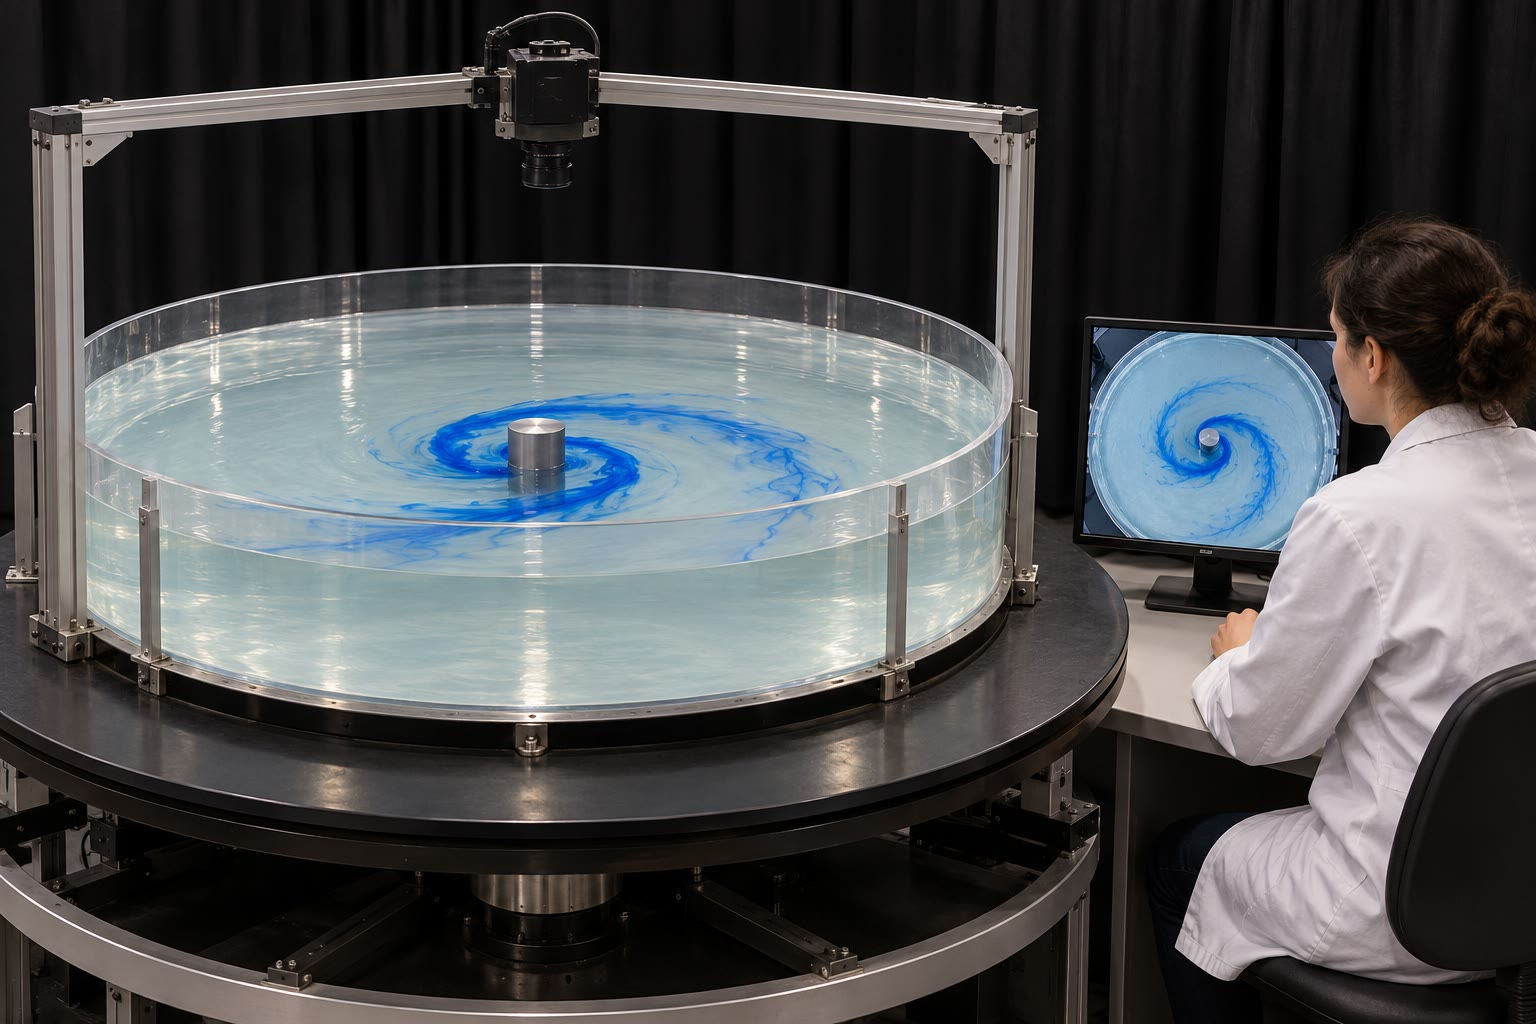
\includegraphics[width=\linewidth]{images/book5/ai/b3-rotating-tank.jpg}

{\scriptsize घूमती टंकी: एक बेलन के चारों ओर सर्पिलाकार घूमता रंजक, उस कैमरे से फ़िल्माया गया जो
थाली के साथ घूमता है (AI से बनाया गया चित्रण)।}
\end{minipage}
\end{inthelab}

\section{अभ्यास}

\begin{exercise}[$\star$]\label{exo:b3:gfd-foundations:1}
मान लीजिए $\Omega = \qty{7.292115e-5}{rad/s}$। (क)~कोरिऑलिस प्राचल और जड़त्वीय आवर्तकाल
\ang{30}, \ang{45} और \ang{60} N अक्षांशों पर परिकलित कीजिए।
(ख)~\qty{0.20}{m/s} की एक धारा के जड़त्वीय वृत्त की त्रिज्या
उन्हीं अक्षांशों पर परिकलित कीजिए। (ग)~\ang{30} पर जड़त्वीय आवर्तकाल की तुलना
नाक्षत्र दिवस \qty{23.9345}{h} से कीजिए।
\end{exercise}

\begin{exercise}[$\star$]\label{exo:b3:gfd-foundations:2}
\ang{45} N पर \omterm{def:b3:gfd-foundations:numbers}{रॉस्बी संख्या} परिकलित कीजिए: धूल-भँवर (\qty{10}{m/s},
\qty{10}{m}), समुद्र समीर (\qty{5}{m/s}, \qty{20}{km}), एक अवदाब
(\qty{15}{m/s}, \qty{1000}{km}) और एक महासागरीय वलय (\qty{0.05}{m/s},
\qty{2000}{km})। इनमें से कौन-से भू-विक्षेपी संतुलन के निकट हैं?
\end{exercise}

\begin{exercise}[$\star$]\label{exo:b3:gfd-foundations:3}
\ang{45} N पर क्षोभमंडल का माध्य तापमान \qty{250}{K} है, जो उत्तर की ओर
प्रति \qty{1000}{km} पर \qty{5}{K} घटता है। ऊँचाई में \omterm{thm:b3:gfd-foundations:thermal-wind}{ऊष्मीय पवन} के पहले पद का उपयोग करके
पश्चिमी पवन का ऊर्ध्वाधर अपरूपण परिकलित कीजिए और
\qty{10}{km} पर पवन में वृद्धि ज्ञात कीजिए।
\end{exercise}

\begin{exercise}[$\star$]\label{exo:b3:gfd-foundations:4}
महासागर के ऊपरी एक किलोमीटर की स्थैतिक स्थिरता $E = -(1/\rho)\,\mathrm d\rho_\theta/\mathrm dz$
का मान \num{50e-8} और \qty{1000e-8}{m^{-1}} के बीच है;
गहरी खाइयों में यह \qty{e-8}{m^{-1}} है। इन तीन मानों के लिए $N = \sqrt{gE}$,
उत्प्लावन दोलन का आवर्तकाल और $N$ प्रति घंटे चक्रों में
परिकलित कीजिए।
\end{exercise}

\begin{exercise}[$\star\star$]\label{exo:b3:gfd-foundations:5}
मान लीजिए एक मौसम तंत्र के लिए $U = \qty{10}{m/s}$, $L = \qty{1000}{km}$, $H =
\qty{10}{km}$, \ang{45} N पर। (क)~इसका ऊर्ध्वाधर वेग और ऊर्ध्वाधर त्वरण आकलित कीजिए,
ऊर्ध्वाधर त्वरण की तुलना $g$ से और
दाब-विक्षोभ की ऊर्ध्वाधर प्रवणता $fUL/H$ से कीजिए। (ख)~लोप किया गया कोरिऑलिस पद
$\tilde fu$ परिकलित कीजिए और इसकी तुलना $g$ से कीजिए।
\end{exercise}

\begin{exercise}[$\star\star$]\label{exo:b3:gfd-foundations:6}
मान लीजिए $f = \qty{e-4}{s^{-1}}$ है और वृत्ताकार समदाब रेखाओं की त्रिज्या
\qty{300}{km} है। (क)~एक निम्न के चारों ओर दाब-प्रवणता $V_g =
\qty{20}{m/s}$ देती है: \omterm{def:b3:gfd-foundations:gradient}{प्रवणता पवन} परिकलित कीजिए। (ख)~एक उच्च के चारों ओर,
$V_g = \qty{5}{m/s}$ के लिए \omterm{def:b3:gfd-foundations:gradient}{प्रवणता पवन} परिकलित कीजिए। (ग)~संभव सबसे बड़ा
$V_g$ कितना है, और तब पवन कितनी होगी?
\end{exercise}

\begin{exercise}[$\star\star$]\label{exo:b3:gfd-foundations:7}
एक टंकी, जो \qty{20}{cm} गहरी है और हर \qty{6}{s} में एक बार घूमती है; उसके पानी की $\nu =
\qty{e-6}{m^2/s}$ है। (क)~$f = 2\Omega$ परिकलित कीजिए, फिर
\qty{5}{cm} चौड़े बेलन के पार \qty{1}{cm/s} के प्रवाह की \omterm{def:b3:gfd-foundations:numbers}{रॉस्बी संख्या}, और
टंकी की \omterm{def:b3:gfd-foundations:numbers}{एकमन संख्या} परिकलित कीजिए। क्या \omterm{thm:b3:gfd-foundations:taylor-proudman}{टेलर स्तंभ} बनेगा? (ख)~सिद्धांत स्पिन-अप
समय $H/\sqrt{\nu\Omega}$ देता है: इसे मिनटों में और थाली के चक्करों में परिकलित कीजिए।
\end{exercise}

\begin{exercise}[$\star\star$]\label{exo:b3:gfd-foundations:8}
1991--2020 के जनवरी आंचलिक माध्य में \ang{30} N पर पश्चिमी पवन \qty{850}{hPa} पर \qty{4.27}{m/s} और
\qty{250}{hPa} पर \qty{40.39}{m/s} है; \ang{45} N पर
\qty{5.99}{m/s} और \qty{23.17}{m/s} है। $R =
\qty{286.9}{J.kg^{-1}.K^{-1}}$ लेकर, दोनों अक्षांशों पर स्तर-माध्य तापमान की
याम्योत्तर प्रवणता परिकलित कीजिए, और बताइए कि जेट
\ang{30} N पर क्यों प्रबल है।
\end{exercise}

\begin{exercise}[$\star\star$]\label{exo:b3:gfd-foundations:9}
(क)~\ang{45} N पर क्षोभमंडल की रॉस्बी त्रिज्या ($N =
\qty{0.0113}{s^{-1}}$, $H = \qty{11}{km}$) और ऊपरी
महासागर की ($N = \qty{0.00357}{s^{-1}}$, $H = \qty{1000}{m}$, \ang{40.5} N) रॉस्बी त्रिज्या परिकलित कीजिए।
(ख)~$a = \qty{6371}{km}$ लेकर, दोनों अक्षांशों पर $\beta$ और
कोरिऑलिस प्राचल का सापेक्ष परिवर्तन $\beta L_R/f$ प्रत्येक त्रिज्या पर परिकलित कीजिए।
\end{exercise}

\begin{exercise}[$\star\star\star$]\label{exo:b3:gfd-foundations:10}
$U$ से गतिमान सतही महासागर का एक जल-पिंड एक रैखिक
घर्षण से मंद होता है: $\mathrm du/\mathrm dt = fv - ru$, $\mathrm dv/\mathrm dt = -fu -
rv$। (क)~$w = u + \mathrm iv$ लेकर हल कीजिए और पथ का वर्णन कीजिए।
(ख)~जल-पिंड एक स्थायी धारा $u_0$ से पूर्व की ओर भी बहता है: इसकी
स्थिति दीजिए। (ग)~\ang{45} N पर $U = \qty{0.2}{m/s}$ और $r^{-1} =
\num{4}\text{ दिन}$ और $u_0 = \qty{0.05}{m/s}$ लेकर, चार दिन बाद धारा के सापेक्ष इसकी चाल
परिकलित कीजिए, और बहकर तय की गई दूरी भी।
\end{exercise}

\begin{exercise}[$\star\star\star$]\label{exo:b3:gfd-foundations:11}
\ang{40} N पर एक महासागरीय अग्र के पार पानी का घनत्व
उत्तर की ओर \qty{100}{km} पर \qty{1}{kg/m^3} बढ़ता है, ऊपरी
\qty{1000}{m} में; नीचे पानी एकसमान और स्थिर है। $\rho_0 =
\qty{1025}{kg/m^3}$ लेकर धारा का ऊर्ध्वाधर अपरूपण और
सतह पर धारा परिकलित कीजिए। यह किस दिशा में बहती है?
\end{exercise}

\begin{exercise}[$\star\star\star$]\label{exo:b3:gfd-foundations:12}
\ang{40.5} N, \ang{30.5} W पर वार्षिक-माध्य स्तंभ के विभव
घनत्व $\sigma_\theta = \rho_\theta - \qty{1000}{kg/m^3}$ के मान सतह पर 26.029,
\qty{100}{m} पर 26.697, \qty{500}{m} पर 27.079 और 27.628
\qty{1000}{m} पर। (क)~तीनों परतों में से प्रत्येक में $N$,
\unit{s^{-1}} में और प्रति घंटे चक्रों में परिकलित कीजिए। (ख)~कौन-सी परत सबसे अधिक स्थिर है,
और क्यों? (ग)~मानों की
\cref{exo:b3:gfd-foundations:4} में दिए ऊपरी महासागर के परास से तुलना कीजिए।
\end{exercise}
% ledger: geod5:grs80-defining, earth:Trot, stewart:stability, data:b5-ncep-uwnd, data:b5-woa23-atlantic, earth:Rmean

\section{समस्या: ओरिन के स्टेपी पर पवनें}

\begin{problem}[{सप्ताहांत समस्या --- घूर्णन, स्तरीकरण और
\ang{48} N पर एक काल्पनिक मैदान की पवनें}]
\label{pb:b3:gfd-foundations:1}
ओरिन का स्टेपी \ang{48} N पर एक समतल मैदान है, जिसमें ओरिन झील है,
\qty{12}{km} चौड़ी, और घूमती टंकी वाली एक छोटी प्रयोगशाला भी है। मान लीजिए
$\Omega = \qty{7.292115e-5}{rad/s}$, $g = \qty{9.81}{m/s^2}$, $R =
\qty{286.9}{J.kg^{-1}.K^{-1}}$ और $c_p = \qty{1004}{J.kg^{-1}.K^{-1}}$।
स्टेपी, उसकी झील और उसकी पवनों के सभी मान काल्पनिक हैं।

\medskip\noindent\textbf{भाग I --- क्या घूर्णन महत्त्वपूर्ण है?}
\begin{enumerate}
\item ओरिन पर कोरिऑलिस प्राचल और जड़त्वीय आवर्तकाल परिकलित कीजिए।
\item पाँच प्रवाहों की \omterm{def:b3:gfd-foundations:numbers}{रॉस्बी संख्या} परिकलित कीजिए: स्नानटब से निकलता पानी
  (\qty{0.1}{m/s}, \qty{0.3}{m} के विस्तार पर); प्रयोगशाला की टंकी, जो
  हर \qty{10}{s} में एक बार घूमती है ($f = 2\Omega_{\text{टंकी}}$ के साथ; \qty{5}{mm/s}
  \qty{0.2}{m} के विस्तार पर); झील से आने वाली शाम की समीर (\qty{5}{m/s},
  \qty{20}{km}); एक अवदाब (\qty{15}{m/s}, \qty{1000}{km}); समान अक्षांश पर किसी महासागरीय द्रोणी का वलय
  (\qty{0.05}{m/s}, \qty{2000}{km})।
\item इनमें से कौन-से प्रवाह उन्हें चलाने वाले घूर्णन का अनुभव करते हैं, और कौन-से
  भू-विक्षेपी के निकट हैं?
\item टंकी (गहराई \qty{0.2}{m}, $\nu =
  \qty{e-6}{m^2/s}$), अवदाब (भँवर श्यानता \qty{10}{m^2/s},
  गहराई \qty{10}{km}) और वलय (भँवर श्यानता \qty{e-3}{m^2/s},
  गहराई \qty{1000}{m}) की \omterm{def:b3:gfd-foundations:numbers}{एकमन संख्या} परिकलित कीजिए।
\item एकमन परत की मोटाई $\delta = \sqrt{2\nu/f}$ है। दिखाइए कि
  $\delta/H = \sqrt{2\,\mathrm{Ek}}$ है, और टंकी तथा
  स्टेपी की हवा के लिए $\delta$ परिकलित कीजिए।
\item इन संख्याओं से पता चलता है कि घर्षण कहाँ महत्त्वपूर्ण है?
\end{enumerate}

\medskip\noindent\textbf{भाग II --- धरातल पर पवन।}
\begin{enumerate}[resume]
\item धरातल पर दाब \qty{1012.9}{hPa} और तापमान
  \qty{288.1}{K} है। हवा का घनत्व परिकलित कीजिए।
\item समुद्र-तल का दाब प्रति
  \qty{300}{km} उत्तर की ओर \qty{4}{hPa} घटता है। भू-विक्षेपी पवन परिकलित कीजिए और उसकी दिशा बताइए।
\item यही प्रवणता एक अवदाब को घेरती है, जिसकी समदाब रेखाओं की त्रिज्या
  \qty{600}{km} है। समदाब रेखाओं की \omterm{def:b3:gfd-foundations:numbers}{रॉस्बी संख्या} और \omterm{def:b3:gfd-foundations:gradient}{प्रवणता पवन}
  परिकलित कीजिए।
\item यही प्रवणता उसी त्रिज्या वाले एक प्रतिचक्रवात को घेरती है।
  \omterm{def:b3:gfd-foundations:gradient}{प्रवणता पवन}, और प्रतिचक्रवात जितनी अधिकतम दाब-प्रवणता धारण कर सकता है, उसे
  \unit{hPa} प्रति \qty{300}{km} में परिकलित कीजिए।
\end{enumerate}

\medskip\noindent\textbf{भाग III --- स्तरीकरण।}
\begin{enumerate}[resume]
\item क्षोभमंडल का तापमान \qty{6.49}{K/km} दर से घटता है।
  शुष्क रुद्धोष्म तापह्रास दर $g/c_p$, तथा $N$ और
  \qty{5}{km} पर उत्प्लावन दोलन का आवर्तकाल, जहाँ तापमान
  \qty{255.7}{K} है, परिकलित कीजिए।
\item \qty{11}{km} के ऊपर हवा \qty{216.6}{K} पर समतापीय है। दिखाइए कि
  वहाँ $N^2 = g^2/(c_pT)$ है, और $N$ तथा
  प्रश्न~11 के मान से उसका अनुपात परिकलित कीजिए।
\item प्रश्न~11 के $N$ और ओरिन के क्षोभमंडल की रॉस्बी त्रिज्या,
  $H = \qty{10}{km}$ लेकर, परिकलित कीजिए और उसकी तुलना
  भाग~I की अवदाब के आकार से कीजिए।
\item गर्मियों में ओरिन झील की ऊपरी \qty{20}{m} परत गहरे पानी से
  \qty{1.5}{kg/m^3} हल्की है ($\rho_0 = \qty{1000}{kg/m^3}$)। न्यून गुरुत्व
  $g' = g\,\Delta\rho/\rho_0$, ऊपरी परत की धीमी आंतरिक तरंगों की
  चाल $\sqrt{g'h}$ और रॉस्बी त्रिज्या
  $\sqrt{g'h}/f$ परिकलित कीजिए।
\item क्या पृथ्वी का घूर्णन झील की आंतरिक गतियों को आकार देगा?
\end{enumerate}

\medskip\noindent\textbf{भाग IV --- ऊष्मीय पवन।}
\begin{enumerate}[resume]
\item एक ही याम्योत्तर पर \qty{600}{km} दूर दो रेडियोसॉन्डे केंद्र हैं।
  धरातल (\qty{1013}{hPa}) से \qty{265}{hPa} तक की परत, जो लगभग
  \qty{10}{km} मोटी है, उसका माध्य तापमान दक्षिणी केंद्र पर \qty{253.0}{K}
  और उत्तरी केंद्र पर \qty{249.4}{K} है। याम्योत्तरीय तापमान-प्रवणता
  \unit{K} प्रति \qty{1000}{km} में परिकलित कीजिए।
\item दो दाबों के बीच की परत की मोटाई $\Delta z = (R\bar
  T/g)\ln(p_b/p_t)$ है। दोनों केंद्रों पर इसका मान, और
  धरातल-स्तर की सतह के सापेक्ष \qty{265}{hPa} सतह की ढाल परिकलित कीजिए।
\item उस ढाल से धरातल से
  \qty{265}{hPa} तक भू-विक्षेपी पवन की वृद्धि निकालिए।
\item \omterm{thm:b3:gfd-foundations:thermal-wind}{ऊष्मीय पवन} प्रमेय (दाब निर्देशांक में) से यही वृद्धि परिकलित कीजिए।
\item क्या स्टेपी की हवा \omterm{def:b3:gfd-foundations:baroclinic}{बैरोट्रॉपिक} है या \omterm{def:b3:gfd-foundations:baroclinic}{बैरोक्लिनिक}? यदि वह \omterm{def:b3:gfd-foundations:baroclinic}{बैरोट्रॉपिक} होती, तो
  \qty{265}{hPa} पर पवन क्या होती?
\item ऊँचाई में \omterm{thm:b3:gfd-foundations:thermal-wind}{ऊष्मीय पवन} के प्रथम पद से वृद्धि,
  मानक क्षोभमंडल का 0 से
  \qty{10}{km} तक का माध्य तापमान \qty{255.7}{K} लेकर, परिकलित कीजिए और तुलना कीजिए।
\item लगभग \qty{5}{km} पर स्थित \qty{541}{hPa} स्तर की पवन
  परिकलित कीजिए, यह मानते हुए कि तापमान-प्रवणता हर स्तर पर एक समान है।
\item रिचर्डसन संख्या $N^2/(\partial u/\partial z)^2$ का मान 0.25 से नीचे
  गिरना चाहिए, तभी अपरूपण प्रक्षुब्धता चला सकता है। ओरिन के क्षोभमंडल के लिए
  इसे परिकलित कीजिए।
\item जनवरी में \qty{250}{hPa} पर आंचलिक माध्य पछुआ पवन \qty{23.2}{m/s} है,
  \ang{45} N पर, और \ang{30} N पर \qty{40.4}{m/s}। ओरिन की पवन से तुलना कीजिए,
  और समझाइए कि स्थानीय पवन आंचलिक माध्य से क्यों अधिक हो सकती है।
\item ओरिन के स्टेपी के ऊपर \qty{10}{km} पर भू-विक्षेपी पवन ज्ञात कीजिए।
\end{enumerate}
\end{problem}
% ledger: geod5:grs80-defining, stewart:stability, data:b5-ncep-uwnd, nasa:grc-atmos
